\documentclass[a4paper,11pt,fleqn]{article}%fleqn pour aligner les equations à gauche
\usepackage{../../Styles/Cours}

\newcommand{\chnum}{Chapitre 3}
\newcommand{\chtitle}{Titrage conductimétrique : les ions chlorure présents dans un lait }
\newcommand{\dtype}{TP}


\begin{document}
\maketitle
\begin{figure}[h!]
	\begin{minipage}{.48\linewidth}
		\textbf{Introduction}\\
		On se propose de déterminer la concentration en masse d’ions chlorure d’un lait maternisé reconstitué.\\
		Le lait maternisé désigne un produit de remplacement partiel ou total du lait maternel. Les laits maternisés contiennent entre autre des ions chlorure \ce{Cl-}, indispensables aux nourrissons\\
		\underline{Normes en vigueur :}
La masse d’ions chlorure doit être comprise entre \num{30} et \SI{112}{mg} pour \SI{100}{mL} de lait reconstitué à \SI{12,9}{\percent} (il s’agit d’un lait en poudre avec lequel on prépare \SI{100}{mL} de lait liquide par dissolution de \SI{12,9}{g} de poudre).
	\end{minipage}\hspace{.02\linewidth}
	\begin{minipage}{.48\linewidth}
		\textbf{Matériel}\\
		\begin{itemize*}
			\item burette graduée de \SI{25}{mL}
			\item agitateur magnétique 
			\item sonde de conductimétrie
			\item balance et sabot de pesée
			\item spatule
			\item éprouvette graduée de \SI{200}{mL}
			\item béchers en verre : \num{2} de \SI{150}{mL} et \num{1} de \SI{400}{mL}
			\item pipette jaugée de 10 mL
			 \item solution de nitrate d’argent de concentration 
		   $c = \SI{10}{\milli\mole\per\liter}$
		\end{itemize*}
	\end{minipage}
\end{figure}

\begin{figure}[h!]
	\begin{minipage}{.48\linewidth}
		\textbf{Protocole expérimental}\\
		\textit{Préparation de l’échantillon à titrer}
		\begin{itemize*}
			\item Peser \SI{1,3}{g} de lait maternisé et introduire l’échantillon dans un bécher de \SI{400}{mL}
			\item Ajouter \SI{200}{mL} d’eau distillée mesurés avec une éprouvette graduée
			\item Agiter jusqu’à dissolution complète
		\end{itemize*}

		\textit{Préparation du montage de titrage}
		\begin{itemize*}
			\item Préparer le dispositif de titrage du bécher précédent par la solution detebtbf nitrate d’argent à \SI{10}{\milli\mole\per\liter}
		\end{itemize*}
		
		\textit{Réalisation du titrage}
		\begin{itemize*}
			\item Relever la première valeur de conductivité pour un volume versé de \SI{0}{mL}.
			\item Poursuivre ainsi en versant la solution titrante \unit{mL} par \unit{mL}.
		\end{itemize*}

		\textit{Exploitation du titrage}
		\begin{itemize*}
			\item Tracer la courbe représentant la conductivité en fonction du volume de solution titrante versé.
			\item Faire les opérations nécessaires pour relever le volume équivalent $V_E$ le plus précisément possible.
		\end{itemize*}
	\end{minipage}\hspace{.02\linewidth}
	\begin{minipage}{.48\linewidth}
		\textbf{Démarche générale}\\
		Les ions chlorure sont titrés avec des ions argent apportés par une solution de nitrate d’argent (\ce{Ag+(aq) + NO3- (aq)}) de concentration apportée ($10 \pm \SI{1}{\milli\mole\per\liter}$). Les ions chlorure et argent réagissent pour former un précipité blanc de chlorure d’argent \ce{AgCl(s)} qui noircit à la lumière.\\
		Le titrage est suivi par conductimétrie afin d’en repérer l’équivalence.\\
		\textbf{Question préliminaire}\\
		Faire un schéma du montage expérimental, en précisant le matériel et les solutions en jeu.
	\end{minipage}
\end{figure}
\section{Exploitation des résultats}
\begin{enumerate}
	\item Établir l’équation de la réaction support de titrage.
	\item Établir la relation à l’équivalence, traduisant l’introduction des réactifs dans les proportions st\oe chiométriques.
	\item Calculer la masse d’ions chlorure $m(\ce{Cl-})$ dans l’échantillon titré et en déduire la masse mX d’ions chlorure dans \SI{100}{g} de lait en poudre. (rapide comparaison avec l’étiquette du flacon au bureau)
	\item Le lait respecte-t-il les normes en vigueur ?
	\item Calculer l’incertitude-type sur la mesure de la masse $m_X$ donnée par la relation :
	$$ u(m_X) = m_X \times \sqrt{\left(\dfrac{u(V_E)}{V_E}\right)^2 + \left(\dfrac{u(m)}{m}\right)^2 + \left(\dfrac{u(c)}{c}\right)^2 + \left(\dfrac{u(M_{Cl})}{M_{Cl}}\right)^2} $$
	Où $V_E$ est le volume équivalent, $m$ la masse de poudre pesée initialement, $c$ la concentration apportée en nitrate d’argent. Les incertitudes-type sur le volume $V_E$  et la masse $m$ seront estimées à partir des instruments de mesure.
	\item Exprimer la masse d’ions chlorure dans l’échantillon titré et en déduire la masse $m_X$ d’ions chlorure dans \SI{100}{g} de lait en poudre sous la forme : $m_X = \overline{m_X} \pm u(m_X)$.
	\item Le résultat du titrage et la valeur indiquée sur l’étiquette du lait maternisé sont-ils compatibles ?
	\item Faire le bilan des ions présents avant et après l’équivalence.
	\item Justifier l’allure de la courbe obtenue.
\end{enumerate}

\textbf{Données :}
\begin{itemize*}
	\item $M(Cl) = \num{35,453} \pm \SI{0,002}{\gram\per\mole}$
	\item Conductivité ionique molaire de quelques ions :
\end{itemize*}
\begin{tabular}{|c|c|c|c|}
	\hline
	ion & \ce{Cl-} & \ce{Ag+} & \ce{NO3-}\\
	\hline
	$\lambda$ en \unit{\milli\siemens\meter\squared\per\mole} & 7.6 & 6.2& 7.1 \\
	\hline	
\end{tabular}

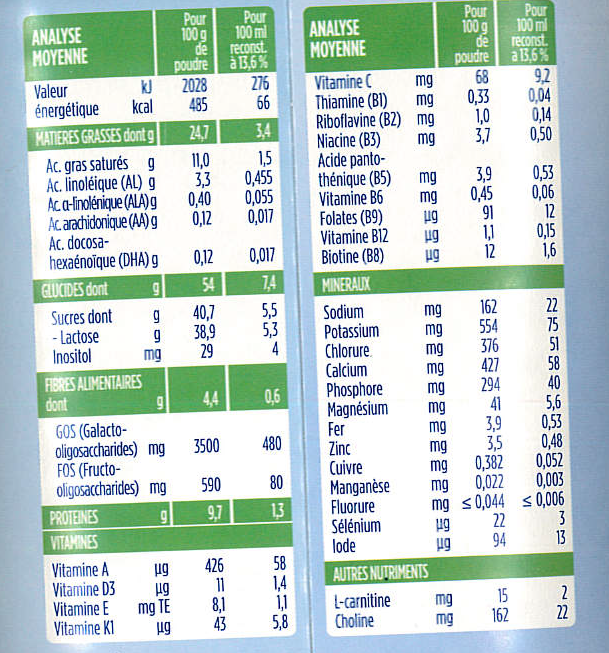
\includegraphics[width = .7\linewidth]{Ressources/TSPE_C2b_AE_Fig1.png}
\end{document}